\documentclass{article}

\usepackage{caption}

\usepackage{enumitem}

\usepackage{graphicx}
\usepackage{float}

\usepackage[
	backend=bibtex
]{biblatex}
\addbibresource{refs.bib}

\captionsetup{
	labelfont=bf,
	font=small,
	justification=centering
}
\renewcommand{\figurename}{Fig.}

\title{
	Canning for Amorphous Blob Computing\\
	\small TER report
}

\author{
    Auteur :\\
    Lucas Labouret\\
    M1 QDCS, Université Paris-Saclay\\
    \small lucas.labouret@universite-paris-saclay.fr
    \and
    Encadrant :\\
    Frédéric Gruau\\
    LISN\\
    \small frederic.gruau@universite-paris-saclay.fr
}

\date{}

\begin{document}
 
\maketitle

\begin{figure}[H]
	\centering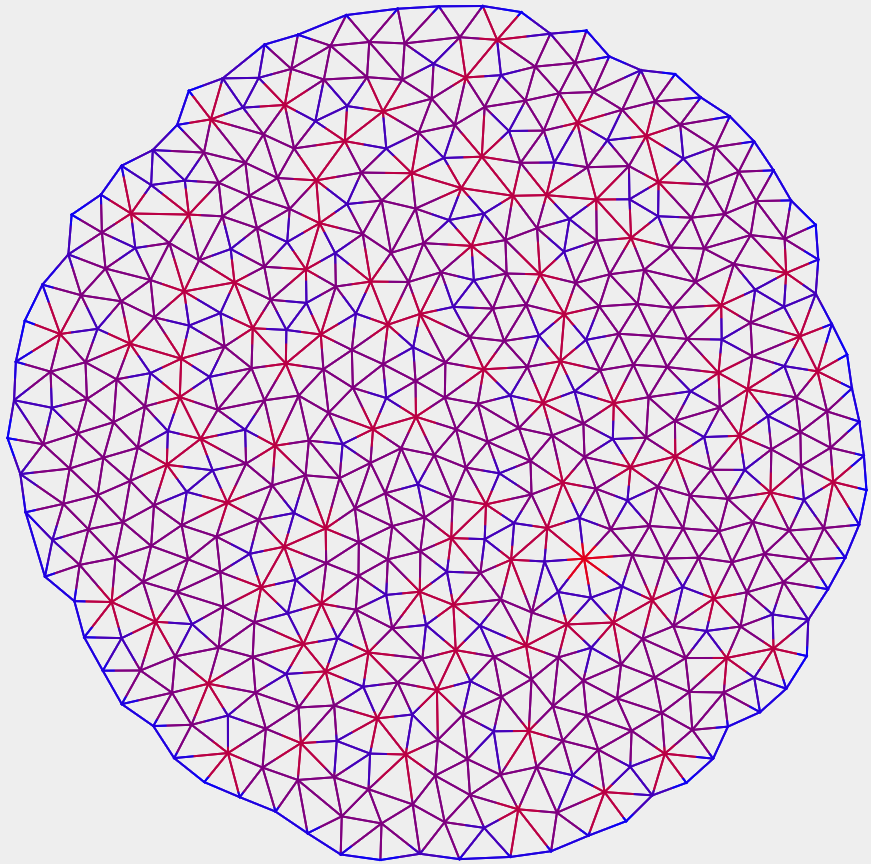
\includegraphics[width=0.9\linewidth]{assets/Circle500.png}
\end{figure}

\newpage
\tableofcontents
\newpage

\renewcommand{\thesection}{\Alph{section}}

\section{What is blob computing ?}

\subsection{Definition and structure of a computing medium}

A computing medium is a weakly Delaunay-triangulated planar graph where each vertex, edge, and face is associated with a "processing element" capable of minimal computation, storing information, and communicating with its neighbors.

\begin{figure}[H]
	\centering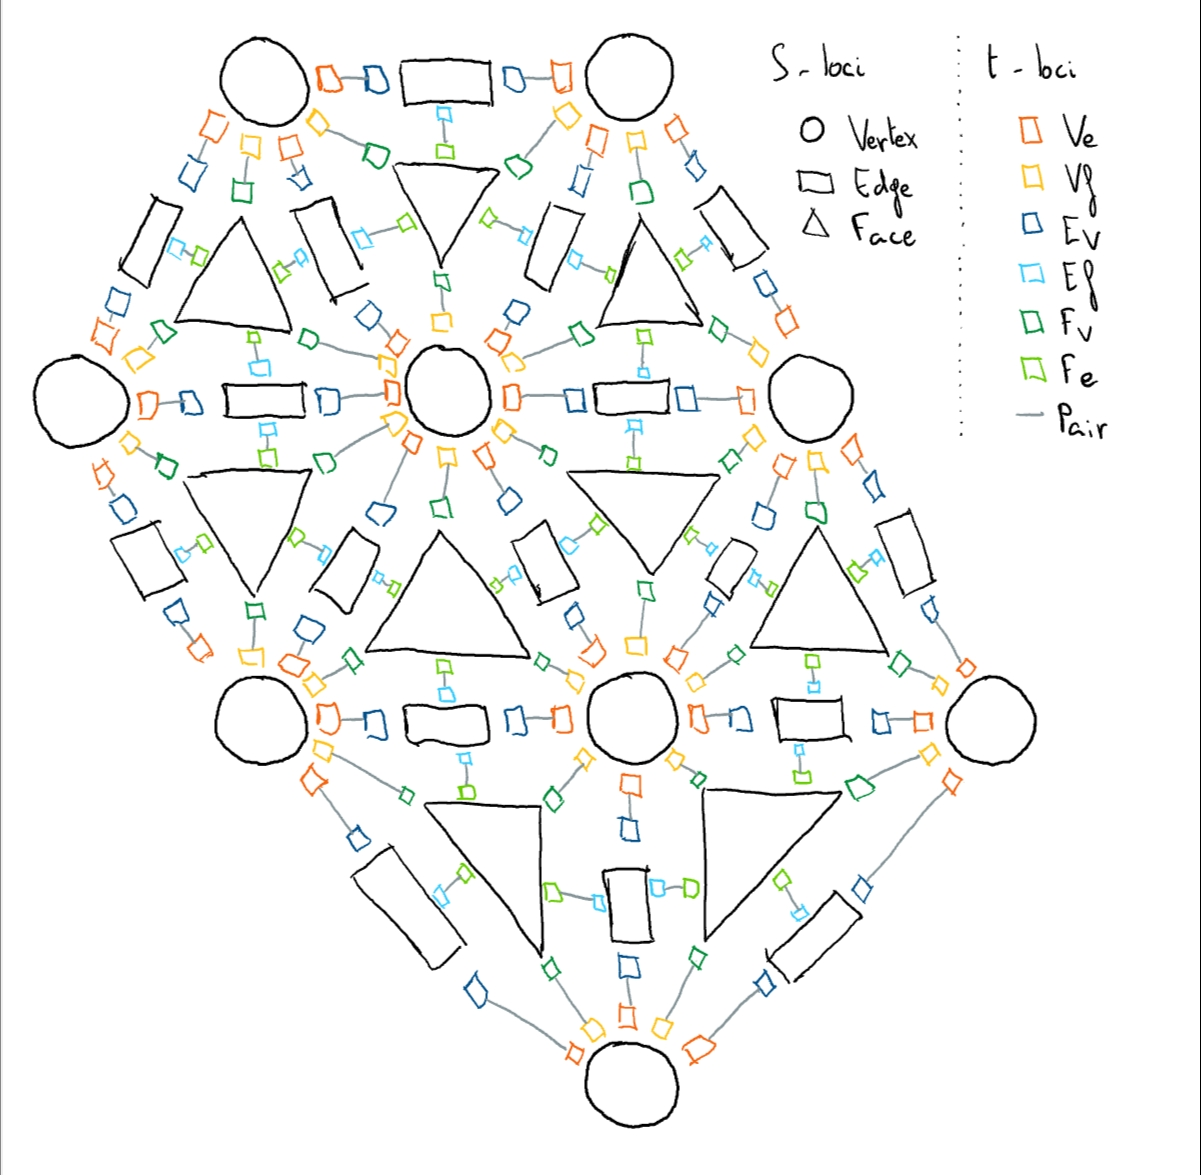
\includegraphics[width=0.9\linewidth]{assets/handdrawn_medium.png}
	\caption{Example structure of a medium.}
	\label{fig:example_structure}
\end{figure}

Vertices, edges and faces are called "simplicial loci" (or "S-loci" for short). They determine the overall structure of their medium. Each S-locus controls a set of "transfer loci" (or "t-loci"). T-loci come in pairs that handle the communication between two S-loci. For example, if a vertex was connected to an edge, there would be a pair of t-loci (one belonging to the vertex and the other belonging to the edge) between them.

Obviously, there are 3 types of S-loci : Vertex, Edge, Face. T-loci are divided into 6 types : 
\begin{itemize}[noitemsep,nosep]
	\item Ve linking a  Vertex to an Edge
	\item Vf linking a  Vertex to a  Face
	\item Ev linking an Edge   to a  Vertex
	\item Ef linking an Edge   to a  Face
	\item Fv linking a  Face   to a  Vertex
	\item Fe linking a  Face   to an Edge
\end{itemize}
Figure~\ref{fig:example_structure} show an example of how all these loci are put together to form a medium.\\

\begin{figure}[H]
	\centering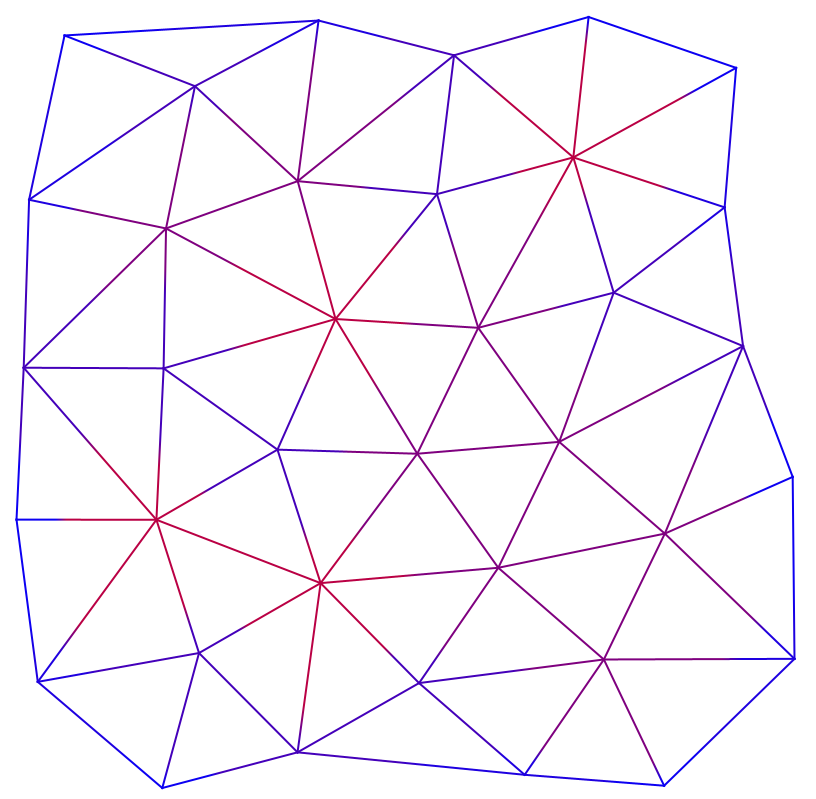
\includegraphics[width=0.4\linewidth]{assets/amorphous_medium.png}
	\hspace{0.1\linewidth}
	\centering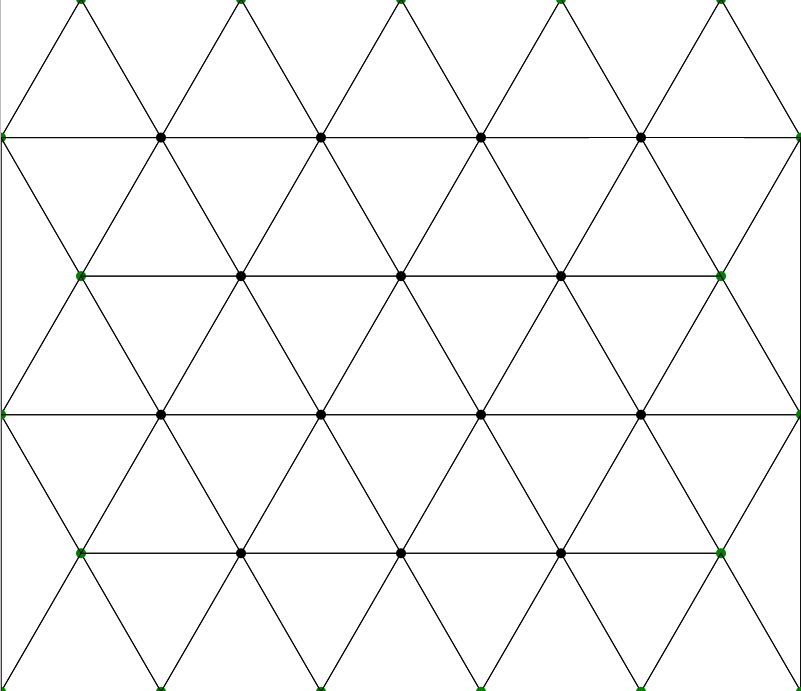
\includegraphics[width=0.4\linewidth]{assets/hexagonal_medium.png}
	\caption{An amorphous isotropic medium (left) VS a crystalline hexagonal medium (right).}
	\label{fig:amorphous_vs_crystaline}
\end{figure}

\subsection{An example of computation : the (discrete) Voronoï diagram}

The article "A parallel data-structure for modular programming of triangulated computing media."\cite{Voronoi} develops tools to program on computing media. As an example, it shows how to build a Voronoï diagram from a set of "seeds" in a medium.

The basic idea is the following : we start with a set of "seeds" distributed over the vertices of the network. Each seed is now the center of a blob. Then, at each synchronous step, the blobs will spread to their adjacent vertices if this wouldn't cause them to merge with another blob, until no blob can spread further. It can be implemented with very few types of local operations that are applied simultaneously to every S-locus in the network :
\begin{itemize}
	\item Multi-cast\\
	The S-locus copies its value into its t-loci of a given type.
	\item Rotation\\
	Since t-loci are spatially arranged around their S-loci, we can define a clockwise and counter-clockwise neighbor. T-loci can perform logical operations on their and their neighbors' values.
	\item Reduction\\
	The S-locus stores the result of a commutative and associative operation applied to the values of its t-loci of a given type.
	\item Transfer\\
	Each of the S-locus' t-loci exchanges its value with the value of its pair. 
\end{itemize}
In fact, clever association of these primitives allows to program everything a computing medium is capable of, such as sorting arrays of integer or multiplying matrices.\cite{other_computation}

\begin{figure}[H]
	\centering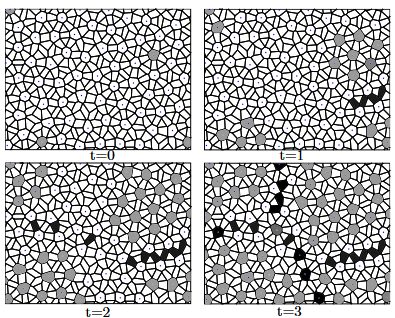
\includegraphics[width=0.7\linewidth]{assets/voronoi_spread.png}
	\caption{
		Computation of a discrete Voronoï diagram.\\
		Cells marked with a dot are the vertices of the medium.
		Gray cells form blobs. Black cells mark the frontiers between blobs. At t=0, blobs only cover the seeds. At t=3, blobs cover Voronoï regions.
	}
	\label{fig:voronoi_spread}
\end{figure}

\subsection{Objective : Cannings}

\section{Preliminary work}

In this section, I detail some work I did last year during another internship with Mr Gruau to generate media with good properties. While it isn't the main focus of this year's interniship, it is what made it possible in its current form.

\subsection{Delaunay Triangulation}

\subsection{Farthest Point Optimization}

The Farthest Point Optimization algorithm \supercite{FPO} allows for the construction of the irregular yet homogeneous sets of points that we need for blob computing.

The implementation of FPO in my case wasn't straightforward. This is because the article applied the algorithm to sets of points in the unit torus, while the media use bounded subsets of the euclidean plane instead. In particular, I had to adapt the algorithm to work around the existence of a border with no predetermined shape, and that can contain fixed points that cannot be moved even though they can still influence the placement of other points.

\renewcommand{\thesection}{\arabic{section}}
\setcounter{section}{0}

\section{GUI}

A large portion of the TER was focused on the development of a graphical interface. It allows to visualize computing media, their optimization through FPO, and the results of different cannings.

\section{Borders and media}

\subsection{Choice of border}

\subsection{Different types of medium}

\section{Canning and evaluation}

\subsection{Partial cannings}

\subsection{Total cannings}

\subsection{Evaluation}

\printbibliography[heading=bibintoc]

\end{document}
